%%%%%%%%%%%%%%%%%%%%%%%%%%%%%%%%%%%%%%%%%%%%%%%%%%%%%%%%%%%%%%
% --> INTRODUCCIÓN
%%%%%%%%%%%%%%%%%%%%%%%%%%%%%%%%%%%%%%%%%%%%%%%%%%%%%%%%%%%%%%
\section{Introducción}

Las pilas y colas son estructuras de datos que se utilizan generalmente para simplificar ciertas operaciones de programación. Estas estructuras pueden implementarse mediante arrays o mediante listas enlazadas. 

Las pilas son estructuras de datos que tienes dos operaciones básicas: push (para insertar un elemento) y pop (para extraer un elemento). Su característica fundamental es que al extraer se obtiene siempre el último elemento que acaba de insertarse. Por esta razón también se conocen como estructuras de datos LIFO (del inglés Last In First Out).Las pilas se utilizan en muchas aplicaciones que utilizamos con frecuencia. Por ejemplo, la gestión de ventanas en Windows (cuando cerramos una ventana siempre recuperamos la que teníamos detrás). Otro ejemplo es la evaluación general de cualquier expresión matemática para evitar tener que calcular el número de variables temporales que hacen falta. Las colas también son llamadas FIFO (First In First Out), que quiere decir \"el primero que entra es el primero que sale\". \cite{R3} 

En este laboratorio se va a trabajar con tipo de estructura de datos para la implementación de funciones básicas y posibles aplicaciones de este tipo de estructuras de datos.

%%%%%%%%%%%%%%%%%%%%%%%%%%%%%%%%%%%%%%%%%%%%%%%%%%%%%%%%%%%%%%
% --> OBJETIVOS
%%%%%%%%%%%%%%%%%%%%%%%%%%%%%%%%%%%%%%%%%%%%%%%%%%%%%%%%%%%%%%
\subsection{Objetivos}



%%%%%%%%%%%%%%%%%%%%%%%%%%%%%%%%%%%%%%%%%%%%%%%%%%%%%%%%%%%%%%
% --> OBJETIVO GENERAL
%%%%%%%%%%%%%%%%%%%%%%%%%%%%%%%%%%%%%%%%%%%%%%%%%%%%%%%%%%%%%%
\subsubsection{Objetivo General}
\begin{itemize}
\item Implementar las estructuras de datos abstractos Stack, Queue utilizando plantillas, herencia y POO en C++, siguiendo el desarrollo hecho en el laboratorio anterior.
\end{itemize}

%%%%%%%%%%%%%%%%%%%%%%%%%%%%%%%%%%%%%%%%%%%%%%%%%%%%%%%%%%%%%%
% --> OBJETIVOS ESPECÍFICOS
%%%%%%%%%%%%%%%%%%%%%%%%%%%%%%%%%%%%%%%%%%%%%%%%%%%%%%%%%%%%%%
\subsubsection{Objetivos Específicos}
\begin{itemize}
\item Implementar una función en C++ que verifique si una hilera de caracteres tiene los paréntesis, llaves y paréntesis cuadrados balanceados.
\item Implementar una función en C++ que simule la operación de un sistema operativo al aten-
der procesos.
\item Utilizar estructuras de datos de pilas (stack) y  colas (queue).
\end{itemize}

%%%%%%%%%%%%%%%%%%%%%%%%%%%%%%%%%%%%%%%%%%%%%%%%%%%%%%%%%%%%%%
% --> ENUNCIADO
%%%%%%%%%%%%%%%%%%%%%%%%%%%%%%%%%%%%%%%%%%%%%%%%%%%%%%%%%%%%%%
\newpage

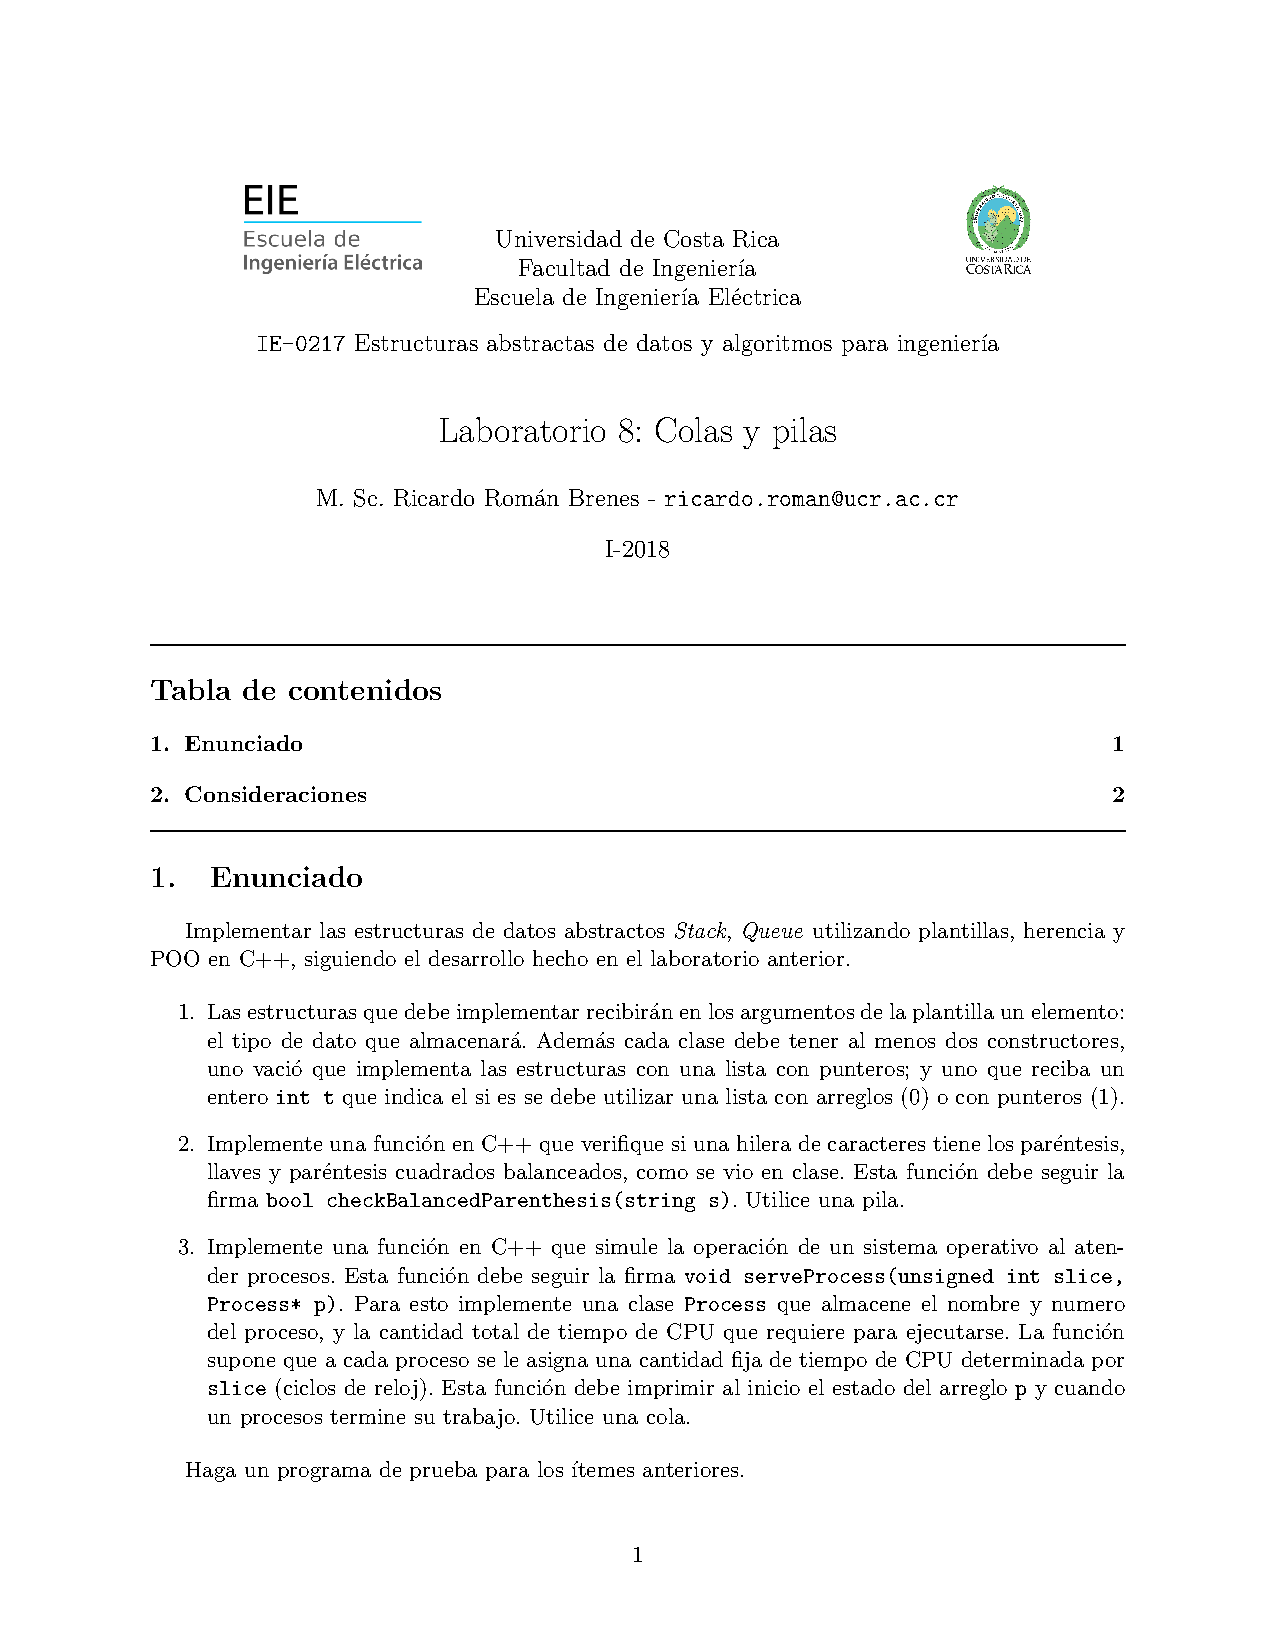
\includepdf[pages=1,pagecommand=\section{Enunciado}, scale=0.8]{enunciados/enun8} 
\includepdf[pages=2,pagecommand={},scale=0.8]{enunciados/enun8}

%%%%%%%%%%%%%%%%%%%%%%%%%%%%%%%%%%%%%%%%%%%%%%%%%%%%%%%%%%%%%%
% --> SOLUCIÓN
%%%%%%%%%%%%%%%%%%%%%%%%%%%%%%%%%%%%%%%%%%%%%%%%%%%%%%%%%%%%%%
\section{Solución}

%--------------------------------------------------------------
\subsection{Cola}
%--------------------------------------------------------------
La cola es un caso especial de una lista con punteros, ya que tiene condiciones especiales que debe cumplir. Una cola tiene una estructura de tipo FIFO (first in first out) es decir, el primer elemento que entra a la estructura es el primer elemento en salir. Por lo tanto, para seguir estas restricciones, utilizando los métodos expuestos en la clase List.h, habrán algunos que no serán implementados pues no tienen sentido en una cola. Por lo tanto se proceden a implementar los siguientes:

\begin{figure}[H]
\centering
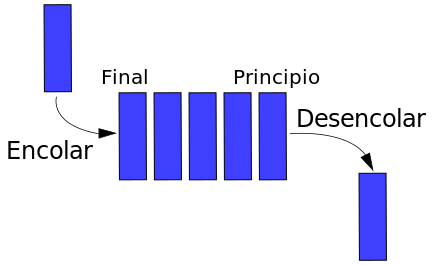
\includegraphics[width=0.35\textwidth]{imgs/Labo8/cola.png}
\caption{Estructura de datos tipo cola}
\label{fig:cola}
\end{figure}

%--------------------------------------------------------------
\subsection{Pila}
%--------------------------------------------------------------

La pila básicamente es una lista con punteros que tiene ciertas restricciones. Una pila es una estructura tipo LIFO (last in first out) de manera entonces que el último elemento que entra es el único que puede salir. Debido a esta restricción entonces limita un poco la implementación de todos los métodos definidos en la clase abstracta List.h que podemos observar en la sección 2.2. Tomando esto en cuenta nos damos que de los métodos virtuales puros solo podemos implementar los siguientes.

\begin{figure}[H]
\centering
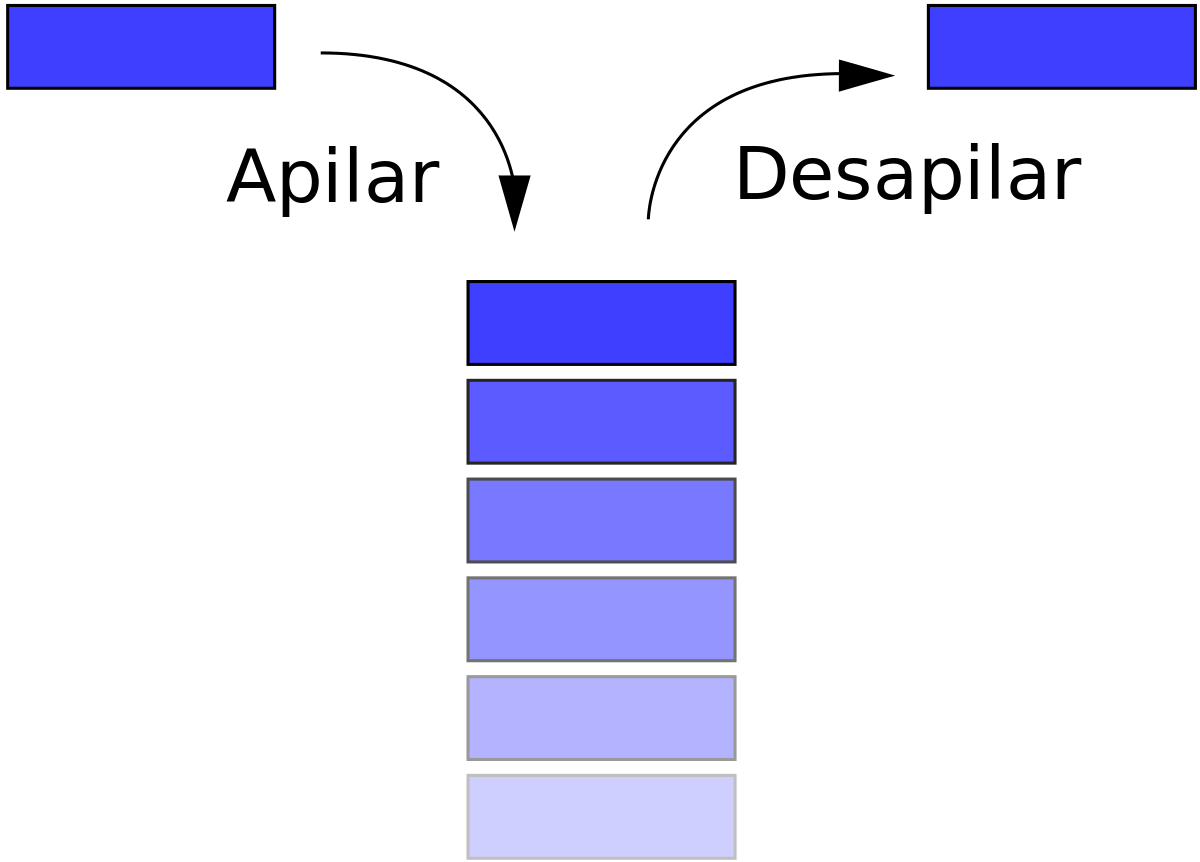
\includegraphics[width=0.35\textwidth]{imgs/Labo8/pila.png}
\caption{Estructura de datos tipo pila}
\label{fig:pila}
\end{figure}



\begin{minted}[linenos,autogobble,bgcolor=bg,breaklines,fontsize=\footnotesize ]{c++}
#include <string>
#include <iostream>
using namespace std;

class FileUtil
{
  public:
  	FileUtil(string s, ios_base::openmode p);
  	~FileUtil();
  	string read();
  	string* readLines();
  	int write(string s);
  	int write(string* s, int n);
    void countNumberLines();
    int getNumberLines();
  private:
    //Numero de lineas.
    int numLines;
    //Dirección de lectura.
    string ruta;
    //Modo de lectura.
  	ios_base::openmode modo;
    //Linea leida.
    string line;
    //Puntero con la direccion del arreglo de las lineas leidas.
    string* lines;

};
\end{minted}



%%%%%%%%%%%%%%%%%%%%%%%%%%%%%%%%%%%%%%%%%%%%%%%%%%%%%%%%%%%%%%
% --> RESULTADOS
%%%%%%%%%%%%%%%%%%%%%%%%%%%%%%%%%%%%%%%%%%%%%%%%%%%%%%%%%%%%%%
\section{Resultados}



%%%%%%%%%%%%%%%%%%%%%%%%%%%%%%%%%%%%%%%%%%%%%%%%%%%%%%%%%%%%%%
% --> CONCLUSIONES
%%%%%%%%%%%%%%%%%%%%%%%%%%%%%%%%%%%%%%%%%%%%%%%%%%%%%%%%%%%%%%
\section{Conclusiones}


Como conclusiones se tiene que:

\begin{itemize}
\item 
\item 
\item 
\item 
\end{itemize}


%%%%%%%%%%%%%%%%%%%%%%%%%%%%%%%%%%%%%%%%%%%%%%%%%%%%%%%%%%%%%%
% --> BIBLIOGRAFIA
%%%%%%%%%%%%%%%%%%%%%%%%%%%%%%%%%%%%%%%%%%%%%%%%%%%%%%%%%%%%%%
\begin{thebibliography}{IEEE}
\bibitem{R1} Talens, S. \textbf{\textit{Curso de programación en C++}}. EUI (UPV) Valencia, 17 al 28 de Julio de 1995. 

\bibitem{R2} Raffo, E. \textbf{\textit{Programación genérica en C++, usando Metaprogramación}}. 2007. Sistemas de Informática. 

\bibitem{R3} Quevedo, E.; López, R. \& Asencio, A. \textbf{\textit{Programación. Tema 4: Pilas y Colas}}. 2014. Sistemas de Informática. 

\end{thebibliography}